\documentclass[journal, a4paper]{IEEEtran}

\usepackage[utf8]{inputenc}

\usepackage[justification=centering]{caption}

\usepackage[left=18mm,right=18mm,top=17mm,bottom=18mm]{geometry}

\setlength{\columnsep}{7mm}

\usepackage{cleveref}

\usepackage[siunitx]{circuitikz}

\usepackage{siunitx}

\usepackage{float}

\usepackage{tikz}

\usetikzlibrary{shapes, arrows}

\usetikzlibrary{shapes.geometric, arrows}

\usetikzlibrary{fit}
\usepackage{multirow}
\usetikzlibrary{scopes}

\usepackage{cite}
\usepackage{graphicx}

\usepackage{url}
\tikzstyle{start} = [circle, draw, centered, fill = white!20, minimum width= 8pt, inner sep= 10pt]
\tikzstyle{decision} =[diamond, draw, fill=white!20, text width= 5em, text centered, node distance = 3cm, inner sep =0pt]
\tikzstyle{common} =[diamond, draw, fill=white!20, text width= 0.5em, text centered, node distance = 3cm, inner sep= 0pt]

\tikzstyle{operation} = [rectangle, draw, fill=white!20, text width = 5em, rounded corners, minimum height=4em ]

\tikzstyle{line} = [draw, -latex']

\tikzstyle{input} = [trapezium, draw, fill=white!20, text width= 4em, minimum height = 4em, trapezium  left angle =120, trapezium right angle = 60]

\setlength\parindent{0pt}

\begin{document}


	\title{ELEN 4020 Lab 3}

	\author{\small Uyanda Mphunga - 1168101 | Darren Blanckensee - 1147279 |
Ashraf Omar - 710435 | Amprayil Joel Oommen - 843463}

	\maketitle

\section{Introduction}
The purpose of this lab is to expose the students to the programming model of MapReduce. MapReduce makes use of underlying principles of parallelization, allowing for large datasets to be processed in a scalable and fault-tolerant way.\\

MapReduce is ordinarily comprised of two types of functions, namely mapping functions and reducing functions (sometimes there are combine functions). The map function operates on every member of an input list, returning as output two linked-pieces of data - a key and a value. These key-value pairs are then grouped according to the keys generated.\\

The output of the map function is then passed on to the reduce function. The reduce function takes in as an argument a key and all values associated with that key, to perform a function set out by the user.\\

For the purposes of this lab, students are required to develop two algorithms which make use of the MapReduce programming model, in order to perform matrix multiplication. Students have opted to make use of Python and the MrJob MapReduce framework, to implement the two algorithms. 

\section{Algorithm A: Naive Matrix Multiplication}
\subsection{Map Function}
\noindent
In order to perform matrix multiplication, the algorithm is required to obtain element data for two matrices (say Matrix A and B) of appropriate size. Hence, when the algorithm is run in the terminal, two input file names are supplied as arguments. Each input file, states the dimensions of a matrix in its first line. This is followed by every single matrix element's coordinate-position as well as value (where the information of each element is on its own newline). This is known as Matrix Market format and is useful for large sparse matrices as there is no need to store elements with value zero.

The map function is designed to read every line of two inputted files. It first determines which input file it has read data from; this information is necessary, since specific logic is employed when generating key value pairs that inserts an 'M' or an 'N' to the value of each key value pair depending on whether the text file is the first text file or the second. For more details about the logic employed, please refer to Figure~\ref{code}. The map function is completed, when a key-value pair is generated for each element of the input files. \\

For Matrix M its elements have coordinates $(i,j)$ where $i$ refers to the rows and $j$ refers to the columns. Matrix M's values are given by $m_{ij}$. For Matrix N its elements have coordinates $(j,k)$ where $j$ refers to the rows and $k$ refers to the columns. Matrix M's values are given by $n_{jk}$. The keys are given by $(i,k)$ where for M $i$ is the $i$ coordinate of element $m_{ij}$ being mapped and $k$ is a value that goes from $0$ to the number of columns of the N matrix. For N $i$ is a value that goes from $0$ to the number of rows of the M matrix and k is the $k$ coordinate of element $n_{jk}$ being mapped. The values for the M matrix are generated in this format $('M' , j , m_{ij})$. The values for the N matrix are generated in this format $('N' , j , n_{jk})$.

	\begin{figure}[hbtp!]
		\centering
		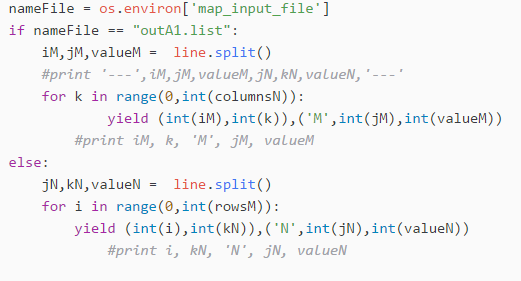
\includegraphics[scale = 0.78]{code.png}
		\caption{Excerpt code}
		\label {code}
	\end{figure}


\subsection{Reduce Function}
\noindent
Once the map function has generated all the key-value pairs for the two matrices, the reduce function is defined to create two lists (one for each matrix) of all the values for each key. These two lists are then sorted according to their $j$ values.
 
 \begin{figure}[hbtp!]
		\centering
		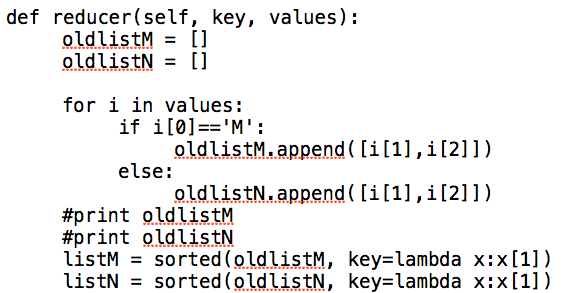
\includegraphics[scale = 0.4]{ListM}
		\caption{List formation}
		\label {code}
	\end{figure}
 
 
\noindent
The matrix multiplication is then performed by calculating the sum of the multiplication of all values $m_{ij}$ and $n_{jk}$ in the lists that have the same $j$ value. This is described by the equation below: 

\begin{center}
$P(i,k) =  \sum_{j}^{n}(m_{ij}*n_{jk})$\\
\end{center}

\noindent
Where $P(i,k)$ is the element in the resulting matrix with coordinates $(i,k)$.
The code implementing the multiplication is shown below:

\begin{figure}[hbtp!]
		\centering
		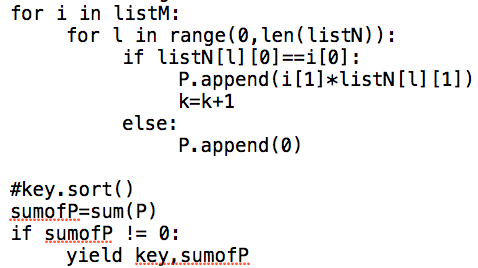
\includegraphics[scale = 0.4]{MM}
		\caption{Matrix Multiplication}
		\label {code}
	\end{figure}
    
\section{Algorithm B}
Due to time constraints, the authors were unable to implement a second algorithm of using MapReduce to perform matrix multiplication. Nonetheless, a second method of performing the matrix multiplication was discovered and its logic shall be presented now. This algorithm, unlike Algorithm A, makes use of two cycles of mapping and reduction, in order to perform matrix multiplication using matrix M with elements $m_{ij}$  and matrix N with elements $n_{ij}$ - i.e. a cycle performing $map$ and $reduce$, followed by a second cycle of $map\_final$ and $reduce\_final$.

\subsection{First MapReduce Cycle}
\noindent
In the first mapping cycle, each matrix element $m_{ij}$ is mapped to its key-value pair of $(j, (M, i, m_{ij}))$ and each matrix element $n_{jk}$ is mapped to its key-value pair of $(j, (N, k, m_{jk}))$. \\

This is followed by a reduction cycle, where for each key $j$, the list of its associated values are considered. For each value of M and N that appears in the key (i.e. $(j, (M, i, m_{ij}))$ and $(j, (M, i, m_{ij}))$), a tuple is created by multiplying the two values, such that $(i, k, v = m_{ij}n_{jk})$.\\

The final output of the reduce function is another set of key-value pairs, in the form of $(j, [ (i_1,k_1,v_1), (i_2,k_2, v_2), ..., (i_p,k_p, v_p) ])$. Thus, these key-value pairs represent all the multiplied pairs that are generated during the matrix multiplication process. The following MapReduce Cycle, is responsible for adding up all the appropriate multiplied pairs.

\subsection{Second MapReduce Cycle}
\noindent
In the second mapping function (i.e. $map\_final$), each of the pairs of the previous reduce function, are mapped to form $p$ key-values (i.e.$((i_1,k_1),v_1), ((i_2,k_2), v_2), ..., ((i_p,k_p), v_p)$ ).

These key-values are inputted into $reduce\_final$, where each $(i,k)$ key is summed, to form the final key-value: $((i,k), v)$. These final key-values, represent the matrix elements of the final multiplied matrix P (where $P=M\times N$).\\

\section{Comparison}

% Please add the following required packages to your document preamble:
% \usepackage{multirow}
% Please add the following required packages to your document preamble:
% \usepackage{multirow}
% Please add the following required packages to your document preamble:
% \usepackage{multirow}
% Please add the following required packages to your document preamble:
% \usepackage{multirow}
\begin{table}[]
\centering
\caption{Table of time comparisons}
\label{my-label}
\begin{tabular}{|l|l|l|l|}
\hline
\multirow{2}{*}{} 
                   & \multicolumn{3}{l|}{Time taken (s)}                  \\ \hline
                  & A1*B1         & A2*B2        & A3*B3        \\ \cline{2-4} 
                 
Algorithm A       & 45.15679            &*              &41.45678              \\ \hline
Algorithm B       &N.A.               &N.A.              &N.A.              \\ \hline
\end{tabular}
\end{table}
Algorithm A was run on the user's computer, as well as on the server provided. It was not able to run for the second set of input files (indicated with a star). Algorithm B has no results, due to the algorithm not being implemented (hence "Not Applicable" is indicated in Table 1).
\section{Directed Graph Problem}

\noindent
A problem is presented in which an unweighted graph $G=(v,e)$ with $|v|$ nodes and $|e|$ edges (of length 1) must be represented in some data structure and then the nodes that are connected by paths of length 3 must be calculated. The most straightforward solution would be to represent the graph as a $v\times v$ matrix with $2\times|e|$ non-zero entries. The each row and each column represent a node and each entry determines connections between the two nodes. A one would mean a direct connection between the two nodes and a zero would mean there is either no connection or it is the same node. In order to see the nodes which are connected by length 2, we multiply the matrix by itself and the non-zero entries are connections of length 2 between the nodes. Therefore, the formula for finding connections of length $n$ between nodes in the graph represented by matrix $G$ is $G^n$. Therefore, to find the connections between nodes of length 3, we need to multiply the matrix by itself 3 times.

	%The result of Figure~\ref{code} is then multiplied with the array that



\section{Conclusion}
Due to time constraints, the lab could not be completed in its entirety. In the report, we have considered the implemented Algorithm A and shown its results in performing Matrix Multiplication for Input files 1 and 3. Algorithm B has not been implemented, but the necessary logic required is presented. The Graph logic is presented, albeit no results have been provided, due to inaccuracy in the outputs generated from the developed code. 

\end{document}